\section{Wyniki badań}

\subsection{Rozwiązanie softwarowe na platformie Arduino}

Przeprowadzono testy polegające na bezpośrednim zliczaniu sygnałów generowanych przez generator zewnętrzy. 
Napięciem, kształtem oraz długością odpowiadały tym produkowanym przez układ RXHDR\_V1.

Przeprowadzono po pięć badań na każdą częstotliwość i wyliczono błąd względem spodziewanego wyniku. 
Czas akwizycji ustalono na jedną sekundę sprawiając że liczba spodziewanych zliczeń jest równa częstotliwości generowanych sygnałów.

Wyniki znajdujące się w tabeli \ref{rts table} zwizualizowane są na wykresie \ref{rts wyniki}.


\begin{figure}[]
        \centering
        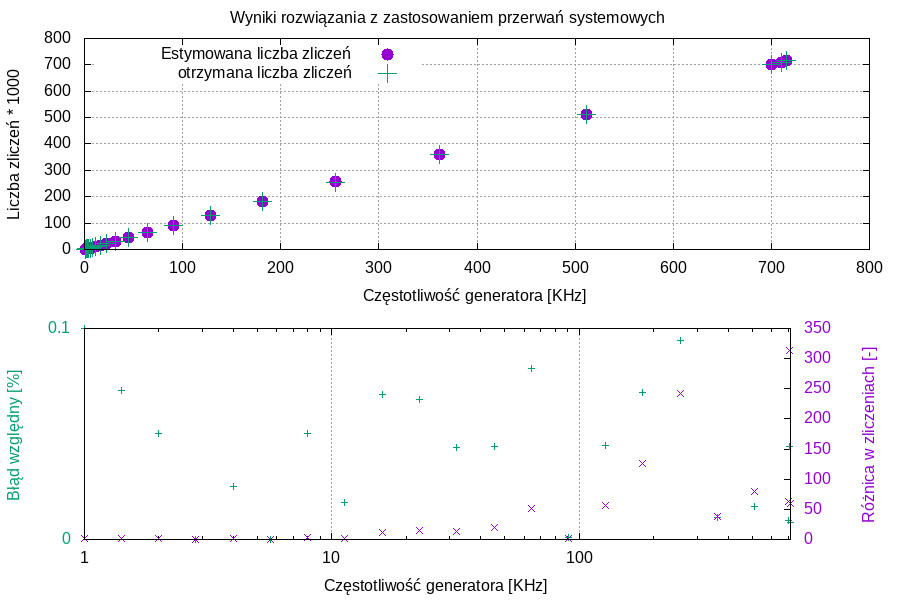
\includegraphics[width=\textwidth]{rts.jpg}
        \caption{Wyniki testów z wykorzystaniem przerwań systemowych}
        \label{rts wyniki}
\end{figure}

\begin{table}
        \centering
        \caption{Wyniki rozwiązania z zastosowaniem przerwań systemowych}
        \label{rts table}
        \begin{tabular}{|c|c|c|c|c|}  
                \hline 
                Częstotliwość [kHz] & Estymowana ilość & Otrzymana ilość & Różnica  & Błąd względny [\%]\\ 
                &  zliczeń &  zliczeń & w zliczeniach & \\ \hline
                1 & 1000 & 1001 & 1 & 0.1000\\ \hline 
                1.414 & 1414 & 1415 & 1 & 0.0707\\ \hline 
                2 & 2000 & 2001 & 1 & 0.0500\\ \hline 
                2.82 & 2820 & 2820 & 0 & 0.0000\\ \hline 
                4 & 4000 & 3999 & 1 & 0.0250\\ \hline 
                5.65 & 5650 & 5650 & 0 & 0.0000\\ \hline 
                8 & 8000 & 7996 & 4 & 0.0500\\ \hline 
                11.3 & 11300 & 11298 & 2 & 0.0177\\ \hline 
                16 & 16000 & 15989 & 11 & 0.0688\\ \hline 
                22.62 & 22620 & 22605 & 15 & 0.0663\\ \hline 
                32 & 32000 & 31986 & 14 & 0.0438\\ \hline 
                45.25 & 45250 & 45230 & 20 & 0.0442\\ \hline 
                64 & 64000 & 63948 & 52 & 0.0813\\ \hline 
                90.5 & 90500 & 90499 & 1 & 0.0011\\ \hline 
                128 & 128000 & 127943 & 57 & 0.0445\\ \hline 
                181 & 181000 & 180874 & 126 & 0.0696\\ \hline 
                256 & 256000 & 255758 & 242 & 0.0945\\ \hline 
                362 & 362000 & 361962 & 38 & 0.0105\\ \hline 
                512 & 512000 & 511920 & 80 & 0.0156\\ \hline 
                700 & 700000 & 699937 & 63 & 0.0090\\ \hline 
                710 & 710000 & 709686 & 314 & 0.0442\\ \hline 
                715 & 715000 & 714941 & 59 & 0.0083\\ \hline
        \end{tabular}
\end{table}

Wyniki pokazują dokładność mieszczącą się w  1\textperthousand, 
jednak błąd w otrzymanym wyniku zależy od częstotliwości generowanych zliczeń.
Może to być spowodowane interferencją przerwania powodującego zliczenie z innymi przerwaniami wymaganymi do działania mikrokontrolera.

Po osiągnięciu częstotliwości granicznej > 0.715 [MHz] program mikrokontrolera przestaje wysyłać dane na komputer zewnętrzny.
Jest to spowodowane tym że zaraz po wyjściu z obsługi przerwania systemowego program natychmiast zaczyna obsługę następnego przerwania. 
Liczba graniczna pozwala przybliżyć czas konieczny na wykonanie jednego przerwania na podstawie przekształcenia wzoru \ref{Cykli w sec}. 
$$ t_p = \frac{1}{f_p} = \sim 1.3986 [\mu s] $$
$$ N_c = \frac{t_p}{t_c} =  \frac{1.3986 \mu s}{11.9 ns} =\sim 118$$
gdzie: \\
        \indent $t_p$ -  czas potrzebny na obsługą przerwania\\
        \indent $t_c$ -  czas jednego cyklu procesora (dział \ref{dzial arduino} ) \\
        \indent $f_p$ -  częstotliwość graniczna przerwań \\
        \indent $N_c$ -  ilość cykli koniecznych na pojedyncze przerwanie \\

Liczba cykli na przerwanie jest mniejsza niż ta szacowana w dziale \ref{dzial arduino} (355 + 128)\cite{ard_opt_git}, wynika to z faktu że poprzednia estymacja była wykonana dla najgorszego przypadku dla nieoptymalizowanego kodu.
Mimo lepszych osiągów niż te szacowane wynik ten nadal odbiega od optymalnego czasu wywołania przerwania (12 + 10) \cite{interupt latency} i wciąż jest znacznie poniżej wymagań projektu. 

Dodatkowe testy potwierdziły że wraz z zwiększeniem ilości badanych kanałów częstotliwość graniczna zmniejsza się jak $\frac{1}{n}$ gdy $n$ to ilość badanych kanałów. 

\subsection{Rozwiązanie z układem zewnętrznych liczników buforujących}

Dane do poniższych wyników zostały uzyskane przez analizę plików archiwalnych otrzymywanych przy działaniu programu do kontroli układu.
Pliki te są przechowywane w formacie JSON.

Analiza sygnałów na oscyloskopie została dokonana na oscyloskopie keysight 3024A. Generator sygnałów używany w układzie badawczym to generator tektonix AFG3102.

Sygnał używany do symulowania impulsów układu RXHDR\_v1 miał wartości 1.8V pick to pick, kształt prostokątny impuls o szerokości 50 us .


\subsubsection{Kalibracja układu}
\label{section kaliblracja}

Przed przystąpieniem do końcowych testów układu konieczne jest przeprowadzenie kalibracji ze względu na uzyskiwany czas martwy układu. 
Oczekiwanym efektem jest regulacja czasu akwizycji w taki sposób że liczba zliczeń będzie odpowiadać ilości impulsów która powinna być uzyskana w czasie akwizycji przez układ bez czasu martwego. 

Zbadano okres jednego cyklu pomiaru (8 kanałów) i uzyskano czas cyklu równy $4.52 \mu s$. Taki cykl jest widoczny na rysunku \ref{Oscyloskop}.
Na podstawie czasu liczby można wyliczyć ilość cykli przypadających na pojedyńcza mikrosekundę.

\begin{equation}
        \label{per cykl}
        CIRCLES\_FOR\_1MS = \frac{1*10^{-3}}{4.52 * 10^{-6}} = 221.238938053
\end{equation}

Korzystając z tej wartości i wartości współczynnika korekcji czasu martwego równego 1 przeprowadzono badania zależności częstotliwości podawanej z generatora do częstotliwości zliczeń dla różnych czasów akwizycji.  

Układ badawczy składał się z komputera, Arduino due, badanego układu elektronicznego, taśmy transmisyjnej, oscyloskopu, generatora impulsów, zasilacza. 

Przeprowadzono trzy badania dla 10 częstotliwości dla 2 czasów akwizycji. Na podstawie tych danych przeprowadzono fitowanie krzywej $f(x) = a*x$ wyniki fitowania umieszczone zostały w tabeli poniżej.

\begin{table}
        \caption{Wyniki fitowania konieczne dla ustalenia korekcji czasu martwego}
        \label{dead time fit}
        \centering
        \begin{tabular}{|c|c|c|c|c|}
                \hline
                Nazwa kanału & czas akwizycji & $a$ & $\Delta a$ & konwersja na 1s \\ \hline
                1A6 & 1000 ms & 0.879395 & $1.893 * 10^{-5}$ & 0.879395 \\ \hline
                2A5 & 500 ms & 0.440366 & $8.156 * 10^{-6}$ & 0.880732 \\ \hline
                2A7 & 500 ms & 0.440352 & $7.939 * 10^{-6}$ & 0.880704 \\ \hline
        \end{tabular}
\end{table}

Na podstawie powyższych danych ustalono wartość współczynnika DEAD\_TIME\_CORECTION równe:
\begin{equation}
        \label{dead time eq}
        DEAD\_TIME\_CORECTION = \frac{1}{\sum^n_i \frac{a_i}{n}} = 1.13636
\end{equation} 

\begin{figure}
        \centering
        \begin{multicols}{2}
                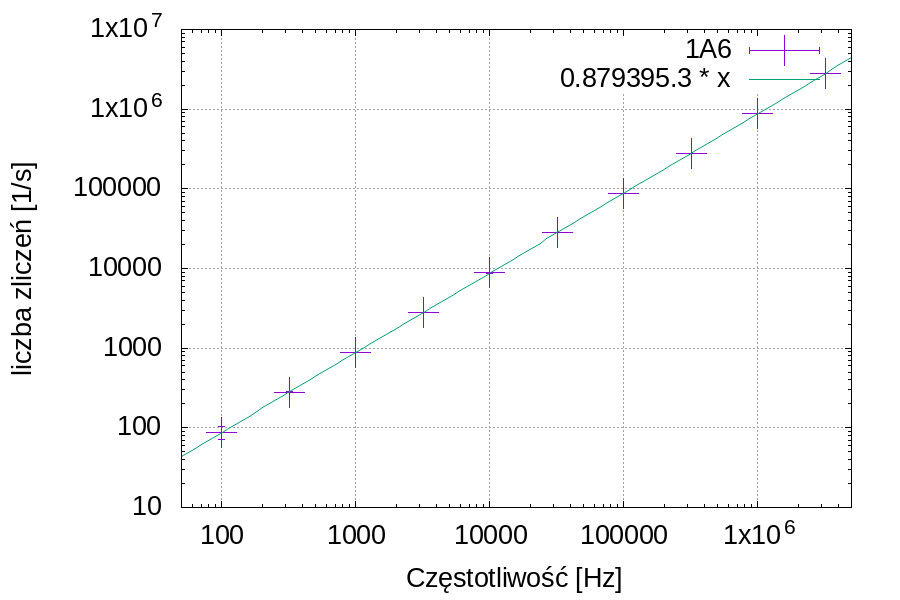
\includegraphics[width=0.45\textwidth]{dead1A6.jpg} \par
                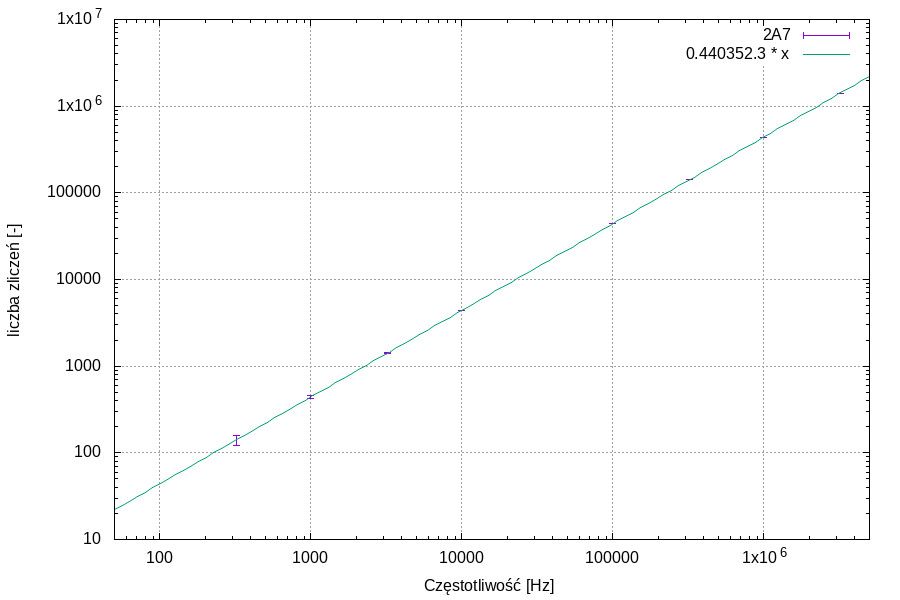
\includegraphics[width=0.45\textwidth]{dead2A7.jpg} \par
        \end{multicols}
        \caption{Wybrane wykresy użyte w celu kalibracji układu}
        \label{wykresy fit calib}
\end{figure}

\subsubsection{Błąd przybliżenia do liczby naturalniej}
Jak widać w fragmencie kodu \ref{code aqw} liczba cykli przeprowadzonych w trakcie pojedyńczej akwizycji musi być liczbą całkowitą. Liczba cykli może być określona wzorem:
\begin{equation}
        N_c [-] = int(A_t*D_t*f_c)
\end{equation}
Gdzie:
\begin{itemize}
        \item $N_c$ - liczba cykli w procesie akwizycji,
        \item $A_t$ - czas  akwizycji w ms
        \item $D_t$ - współczynnik korekcji czasu martwego 
        \item $f_c$ - ilość cykli w ms
\end{itemize}

Błąd wprowadzony w wyniku przybliżenia mieści się w przedziale wartości [0,1) pozwala to na wyliczenie maksymalnego względnego błędu uzyskiwanego w wyniku przybliżania:
\begin{equation}
        \Delta N_{c_{max}} [\%] = \frac{1}{A_t*D_t*f_c}  * 100\%
\end{equation} 
Gdzie:
\begin{itemize}
        \item $\Delta N_{c_{max}}$ - maksymalny względny błąd,
        \item $A_t$ - czas  akwizycji w ms
        \item $D_t$ - współczynnik korekcji czasu martwego 
        \item $f_c$ - ilość cykli w ms
\end{itemize}

Podstawiając współczynniki uzyskane w dziale \ref{section kaliblracja} możemy uzyskać wartości maksymalnego błędu dla najczęściej używanych czasów akwizycji. Wartości te znajdują się w tabeli \ref{tab przyblizenie niep}. Na podstawie tych wartości można stwierdzić że błąd popełniony podczas przybliżania zmienia się w zależności od czasu akwizycji jest on jednak pomijalnie mały.

\begin{table}
        \centering
        \caption{Wartości błędu wynikające z przybliżenia liczbą całkowitą}
        \label{tab przyblizenie niep}
        \begin{tabular}{|c|c||c|c|}
                \hline
                Czas akwizycji [ms] &   $\Delta N_{c_{max}} [\%]$&Czas akwizycji [ms] &   $\Delta N_{c_{max}} [\%]$ \\ \hline
                50 & 0.007955 & 100 & 0.003977 \\ \hline
                1000 & 0.0003977 & 5000 & 0.00007955 \\ \hline
        \end{tabular}
\end{table}

\subsubsection{Testowanie układu liczników za pomocą generatora zewnętrzego.}

Przy wykorzystaniu współczynników otrzymanych w dziale \ref{section kaliblracja} przeprowadzono test układu z wykorzystaniem dzielnika pozwalającego na dostarczenie sygnałów impulsów odpowiadającym tym generowanym przez układ RXHDR\_V1 do wszystkich kanałów jednocześnie. 